% Options for packages loaded elsewhere
\PassOptionsToPackage{unicode}{hyperref}
\PassOptionsToPackage{hyphens}{url}
\documentclass[
]{article}
\usepackage{xcolor}
\usepackage[margin=1in]{geometry}
\usepackage{amsmath,amssymb}
\setcounter{secnumdepth}{5}
\usepackage{iftex}
\ifPDFTeX
  \usepackage[T1]{fontenc}
  \usepackage[utf8]{inputenc}
  \usepackage{textcomp} % provide euro and other symbols
\else % if luatex or xetex
  \usepackage{unicode-math} % this also loads fontspec
  \defaultfontfeatures{Scale=MatchLowercase}
  \defaultfontfeatures[\rmfamily]{Ligatures=TeX,Scale=1}
\fi
\usepackage{lmodern}
\ifPDFTeX\else
  % xetex/luatex font selection
\fi
% Use upquote if available, for straight quotes in verbatim environments
\IfFileExists{upquote.sty}{\usepackage{upquote}}{}
\IfFileExists{microtype.sty}{% use microtype if available
  \usepackage[]{microtype}
  \UseMicrotypeSet[protrusion]{basicmath} % disable protrusion for tt fonts
}{}
\makeatletter
\@ifundefined{KOMAClassName}{% if non-KOMA class
  \IfFileExists{parskip.sty}{%
    \usepackage{parskip}
  }{% else
    \setlength{\parindent}{0pt}
    \setlength{\parskip}{6pt plus 2pt minus 1pt}}
}{% if KOMA class
  \KOMAoptions{parskip=half}}
\makeatother
\usepackage{longtable,booktabs,array}
\usepackage{calc} % for calculating minipage widths
% Correct order of tables after \paragraph or \subparagraph
\usepackage{etoolbox}
\makeatletter
\patchcmd\longtable{\par}{\if@noskipsec\mbox{}\fi\par}{}{}
\makeatother
% Allow footnotes in longtable head/foot
\IfFileExists{footnotehyper.sty}{\usepackage{footnotehyper}}{\usepackage{footnote}}
\makesavenoteenv{longtable}
\usepackage{graphicx}
\makeatletter
\newsavebox\pandoc@box
\newcommand*\pandocbounded[1]{% scales image to fit in text height/width
  \sbox\pandoc@box{#1}%
  \Gscale@div\@tempa{\textheight}{\dimexpr\ht\pandoc@box+\dp\pandoc@box\relax}%
  \Gscale@div\@tempb{\linewidth}{\wd\pandoc@box}%
  \ifdim\@tempb\p@<\@tempa\p@\let\@tempa\@tempb\fi% select the smaller of both
  \ifdim\@tempa\p@<\p@\scalebox{\@tempa}{\usebox\pandoc@box}%
  \else\usebox{\pandoc@box}%
  \fi%
}
% Set default figure placement to htbp
\def\fps@figure{htbp}
\makeatother
% definitions for citeproc citations
\NewDocumentCommand\citeproctext{}{}
\NewDocumentCommand\citeproc{mm}{%
  \begingroup\def\citeproctext{#2}\cite{#1}\endgroup}
\makeatletter
 % allow citations to break across lines
 \let\@cite@ofmt\@firstofone
 % avoid brackets around text for \cite:
 \def\@biblabel#1{}
 \def\@cite#1#2{{#1\if@tempswa , #2\fi}}
\makeatother
\newlength{\cslhangindent}
\setlength{\cslhangindent}{1.5em}
\newlength{\csllabelwidth}
\setlength{\csllabelwidth}{3em}
\newenvironment{CSLReferences}[2] % #1 hanging-indent, #2 entry-spacing
 {\begin{list}{}{%
  \setlength{\itemindent}{0pt}
  \setlength{\leftmargin}{0pt}
  \setlength{\parsep}{0pt}
  % turn on hanging indent if param 1 is 1
  \ifodd #1
   \setlength{\leftmargin}{\cslhangindent}
   \setlength{\itemindent}{-1\cslhangindent}
  \fi
  % set entry spacing
  \setlength{\itemsep}{#2\baselineskip}}}
 {\end{list}}
\usepackage{calc}
\newcommand{\CSLBlock}[1]{\hfill\break\parbox[t]{\linewidth}{\strut\ignorespaces#1\strut}}
\newcommand{\CSLLeftMargin}[1]{\parbox[t]{\csllabelwidth}{\strut#1\strut}}
\newcommand{\CSLRightInline}[1]{\parbox[t]{\linewidth - \csllabelwidth}{\strut#1\strut}}
\newcommand{\CSLIndent}[1]{\hspace{\cslhangindent}#1}
\setlength{\emergencystretch}{3em} % prevent overfull lines
\providecommand{\tightlist}{%
  \setlength{\itemsep}{0pt}\setlength{\parskip}{0pt}}
\renewcommand{\contentsname}{Tabla de contenidos}
\usepackage{float}
\usepackage{booktabs}
\usepackage{bookmark}
\IfFileExists{xurl.sty}{\usepackage{xurl}}{} % add URL line breaks if available
\urlstyle{same}
\hypersetup{
  pdftitle={Reporte de Proyecto},
  pdfauthor={José Carlos Quintero; Paola Espinoza; Julián Soto; María Paula Jiménez},
  hidelinks,
  pdfcreator={LaTeX via pandoc}}

\title{Reporte de Proyecto}
\author{José Carlos Quintero \and Paola Espinoza \and Julián
Soto \and María Paula Jiménez}
\date{3 de octubre de 2025}

\begin{document}
\maketitle

{
\setcounter{tocdepth}{2}
\tableofcontents
}
\section{Resumen}\label{resumen}

Este estudio analiza la prevalencia de sobrepeso y obesidad infantil en
Costa Rica a partir del Primer Censo Escolar de Peso/Talla 2016 (niños
de 6 a 12 años). Se modelan los conteos de casos por cantón mediante un
modelo binomial con enlace logit e inferencia bayesiana, incorporando
covariables socioeconómicas y demográficas estandarizadas. La estimación
se realiza con el algoritmo No-U-Turn Sampler (NUTS), que permite
obtener distribuciones posteriores bien mezcladas para las
probabilidades de prevalencia en cada unidad territorial. A nivel
nacional, la media posterior de obesidad es cercana al 14 \% y la de
sobrepeso al 20 \%, lo que implica un exceso de peso combinado de
alrededor del 34 \%. Se observa un gradiente centro--periferia:
provincias y cantones del Valle Central presentan las prevalencias más
elevadas, mientras que zonas costeras y periféricas muestran valores
sistemáticamente menores. Los resultados confirman que el exceso de peso
infantil constituye un problema estructural de salud pública y muestran
que el enfoque bayesiano logit--binomial es útil para cuantificar la
prevalencia y su incertidumbre a distintos niveles geográficos.

\emph{Palabras clave:} Costa Rica, sobrepeso, obesidad

\section{Introducción}\label{introducciuxf3n}

El sobrepeso y la obesidad infantil se han consolidado en las últimas
décadas como una de las principales problemáticas de salud pública a
nivel mundial: entre 1975 y 2016 el número de niños y adolescentes con
obesidad se multiplicó por más de diez, y más de 200 millones
presentaban sobrepeso (\citeproc{ref-WHO2018}{World Health Organization,
2018}). Estas condiciones se asocian con complicaciones metabólicas y
psicosociales en la niñez y con un mayor riesgo de enfermedad crónica,
discapacidad y mortalidad prematura en la adultez
(\citeproc{ref-Gamboa2021}{Gamboa-Gamboa et al., 2021}).

En Costa Rica, el Primer Censo Escolar de Peso/Talla 2016 reveló que más
de un tercio de los escolares presenta exceso de peso
(\citeproc{ref-Gomez2023}{Gómez et al., 2023}). Estudios nacionales han
mostrado que la prevalencia es mayor en varones, en escuelas privadas y
en distritos urbanos con mayor desarrollo socioeconómico
(\citeproc{ref-Gamboa2021}{Gamboa-Gamboa et al., 2021}), y que las
curvas nacionales de índice de masa corporal (IMC) y circunferencia de
cintura difieren de los patrones internacionales
(\citeproc{ref-Nunez2022}{Núñez-Rivas et al., 2022}), lo que subraya la
necesidad de contar con referencias y análisis propios. A nivel
regional, trabajos como Hernández-Vásquez et al.
(\citeproc{ref-Hernandez2016}{2016}) para Perú y Gómez et al.
(\citeproc{ref-Gomez2023}{2023}) para Costa Rica indican que el
sobrepeso y la obesidad infantil tienden a concentrarse en territorios
urbanos y costeros, evidenciando un componente territorial y
socioeconómico en su distribución.

En este marco teórico, el problema se concibe como un fenómeno de
prevalencia territorialmente heterogénea, influido por factores
demográficos, económicos y de urbanización. Resulta necesario no solo
estimar la magnitud del sobrepeso y la obesidad, sino también
cuantificar rigurosamente la incertidumbre asociada a esas estimaciones
y describir su patrón espacial en el país.

Este panorama motiva la siguiente pregunta de investigación:
\textbf{¿cómo se distribuye territorialmente la prevalencia de sobrepeso
y obesidad infantil en Costa Rica, y con qué grado de incertidumbre
podemos estimarla a partir de la evidencia disponible?} Para
responderla, se adopta un enfoque bayesiano que modela los conteos de
casos mediante un modelo binomial con enlace logit, incorpora
covariables sociodemográficas y utiliza algoritmos de muestreo tipo
HMC/NUTS (\citeproc{ref-HoffmanGelman2014}{Hoffman \& Gelman, 2014})
para aproximar la distribución posterior. A partir de estas
distribuciones posteriores se comparan provincias y cantones mediante
medias e intervalos de credibilidad, y se construyen mapas y gráficos
que permiten interpretar la heterogeneidad territorial y apoyar el
diseño de políticas públicas basadas en evidencia.

\section{Metodología}\label{metodologuxeda}

\subsection{Descripción de los datos}\label{descripciuxf3n-de-los-datos}

La base de datos empleada contiene indicadores socioeconómicos y
demográficos por distrito, así como medidas de prevalencia de sobrepeso
y obesidad infantil. La fuente primaria de información es el Primer
Censo Escolar Peso/Talla del 2016, una iniciativa que recolectó datos
antropométricos de 347.379 niños entre 6 y 12 años pertenecientes al
sistema escolar público y privado de Costa Rica. La información se
encuentra desagregada en unidades administrativas (provincias, cantones
y distritos). Para este estudio se seleccionaron las provincias como
unidad de análisis.

Las variables consideradas en el análisis se describen a continuación:

\begin{itemize}
\item
  \textbf{distrito}: Nombre del distrito al que corresponde el registro.
\item
  \textbf{provincia}: Nombre de la provincia correspondiente.
\item
  \textbf{canton}: Nombre del cantón correspondiente. Representa la
  unidad territorial principal de análisis.
\item
  \textbf{condicion}: Clasificación de los casos según el estado
  nutricional: sobrepeso, obesidad o combinada.
\item
  \textbf{total}: Total de personas observadas.
\item
  \textbf{subtotal}: Número de casos registrados por cantón dentro de
  cada categoría específica de condición.
\item
  \textbf{prevalencia}: Porcentaje de la población del cantón que
  presenta sobrepeso, obesidad o ambas.
\item
  \textbf{desempleo}: Porcentaje de personas desempleadas dentro del
  cantón.
\item
  \textbf{poblacion\_urbana}: Porcentaje de la población que reside en
  áreas urbanas del cantón.
\item
  \textbf{privacion\_critica}: Porcentaje de población en situación de
  privación crítica.
\item
  \textbf{poblacion\_menor\_14}: Porcentaje de personas menores de 14
  años en la población total del cantón.
\item
  \textbf{hogares\_monomarentales}: Porcentaje de hogares encabezados
  por un solo padre o madre.
\item
  \textbf{ocupantes\_por\_hogar}: Promedio de personas que habitan en
  cada hogar del cantón.
\item
  \textbf{anos\_escolaridad}: Promedio de años de escolaridad alcanzados
  por la población, indicador del nivel educativo.
\end{itemize}

\subsection{Análisis exploratorio de la base de
datos}\label{anuxe1lisis-exploratorio-de-la-base-de-datos}

En términos generales, la prevalencia combinada de sobrepeso y obesidad
infantil muestra una media del 34\%, con valores entre 13\% y 56\%,
reflejando una variabilidad importante entre distritos. Al desagregar,
la prevalencia de sobrepeso presenta un promedio de 20\%, con una
desviación estándar del 3\% y un rango entre 6 y 33\%, mientras que la
prevalencia de obesidad registra un promedio de 14\%, con desviación
estándar del 4\% y valores entre 0 y 33\%. Estos resultados evidencian
que, aunque ambas condiciones están presentes en magnitudes
considerables, el sobrepeso es más frecuente que la obesidad, lo cual no
es sorprendente al considerar que la obesidad se puede interpretar como
un caso extremo de sobrepeso.

Los años de escolaridad promedio por distrito se sitúan en 8.1 años, con
una dispersión moderada \(sd \approx 1.5\). La tasa de desempleo es baja
en promedio (3\%), pero con algunos distritos alcanzando valores
cercanos a 9\%. El porcentaje de hogares monomarentales ronda el 20\% y
la privación crítica promedio de los hogares se ubica en 29\%, mostrando
casos extremos de hasta 90\% La población urbana evidencia una clara
polarización: muchos distritos son predominantemente rurales (0\%) o
completamente urbanos (100\%).

\subsubsection{Enfoque Bayesiano}\label{enfoque-bayesiano}

Dada la naturaleza de los datos, se modela el número total de casos
observados en cada categoría (sobrepeso y obesidad, respectivamente)
mediante una distribución \(Y \sim \text{Binom}(N,p)\), donde \(Y\) es
el número total de casos, N el tamaño de la muestra y \(p\) la
probabilidad de pertenecer a la categoría de sobrepeso (o bien,
obesidad) independientemente de la pertenencia provincial o cantonal.
Desde un enfoque bayesiano, se asigna una distribución previa
\(\pi \sim \text{Beta}(1,1)\). De esta forma, se estima la prevalencia
de obesidad y sobrepeso infantil en Costa Rica, a través del algoritmo
Metropolis-Hastings.

\paragraph{Autocorrelación e
Histogramas}\label{autocorrelaciuxf3n-e-histogramas}

Para el método de Metropolis-Hasting, en ambos casos, se obtuvo una alta
autocorrelación entre los elementos de la cadena. Una vez finalizado el
proceso, se realizaron histogramas para visualizar la distribución
posterior obtenida a partir de esta metodología. Además, se presenta la
media y el intervalo de confianza para cada categoría.

\begin{figure}[H]

{\centering 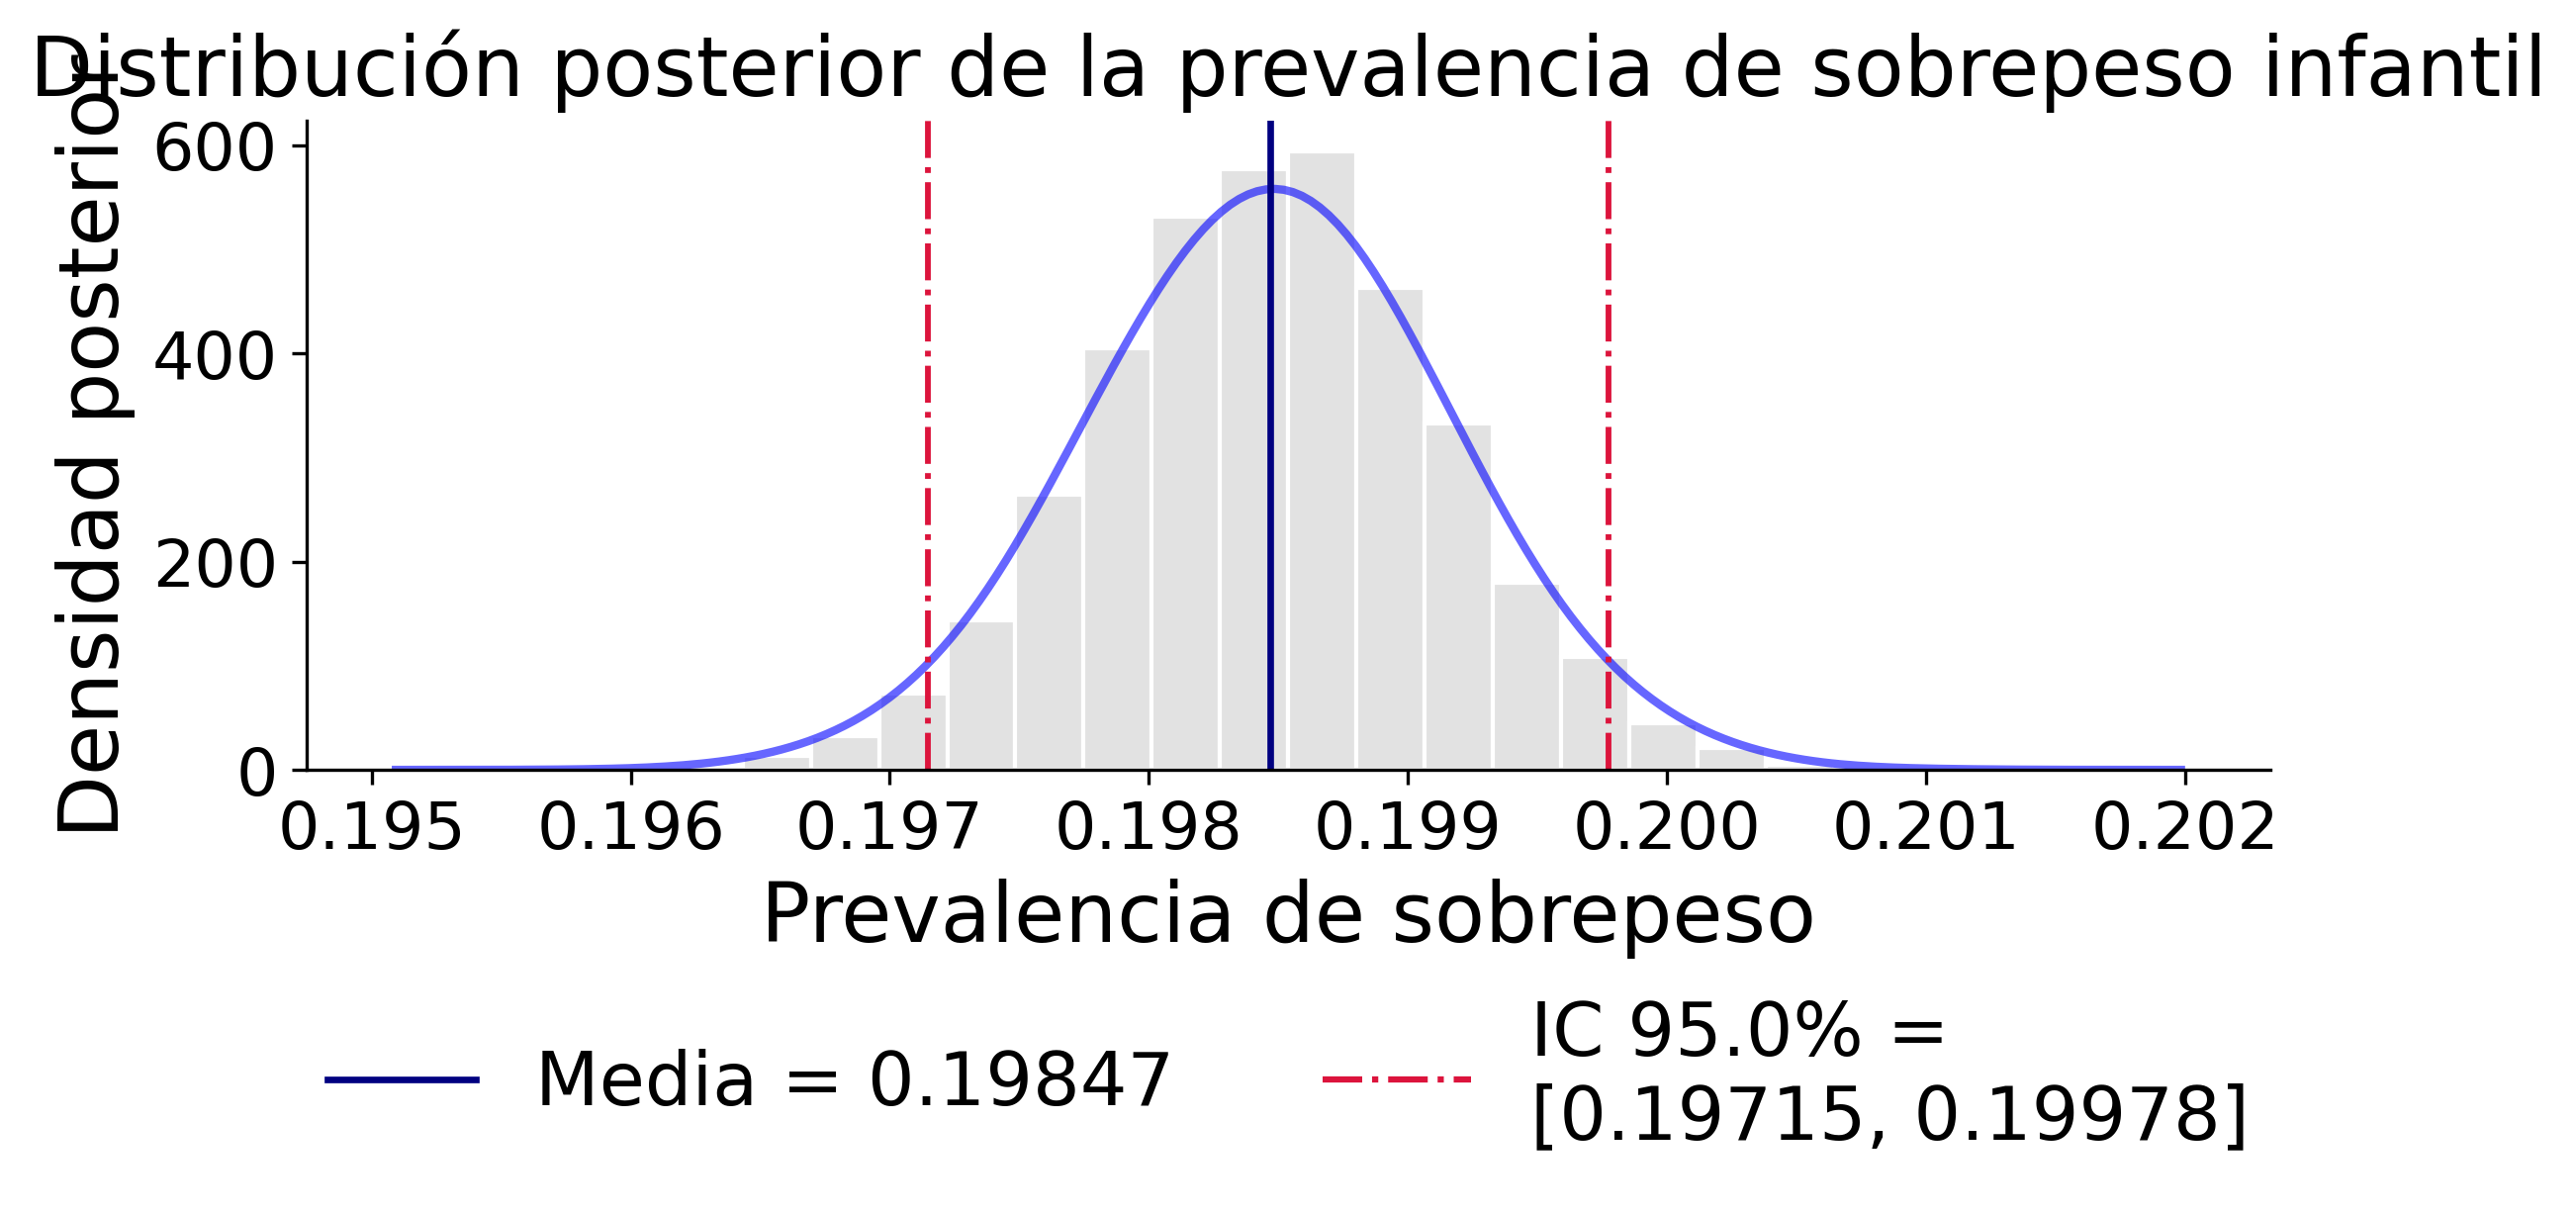
\includegraphics[width=0.7\linewidth]{../res/graficos/hist_post_sobrepeso} 

}

\caption{Distribución posterior de la prevalencia de sobrepeso infantil}\label{fig:fig-sobpreso}
\end{figure}

\begin{figure}[H]

{\centering 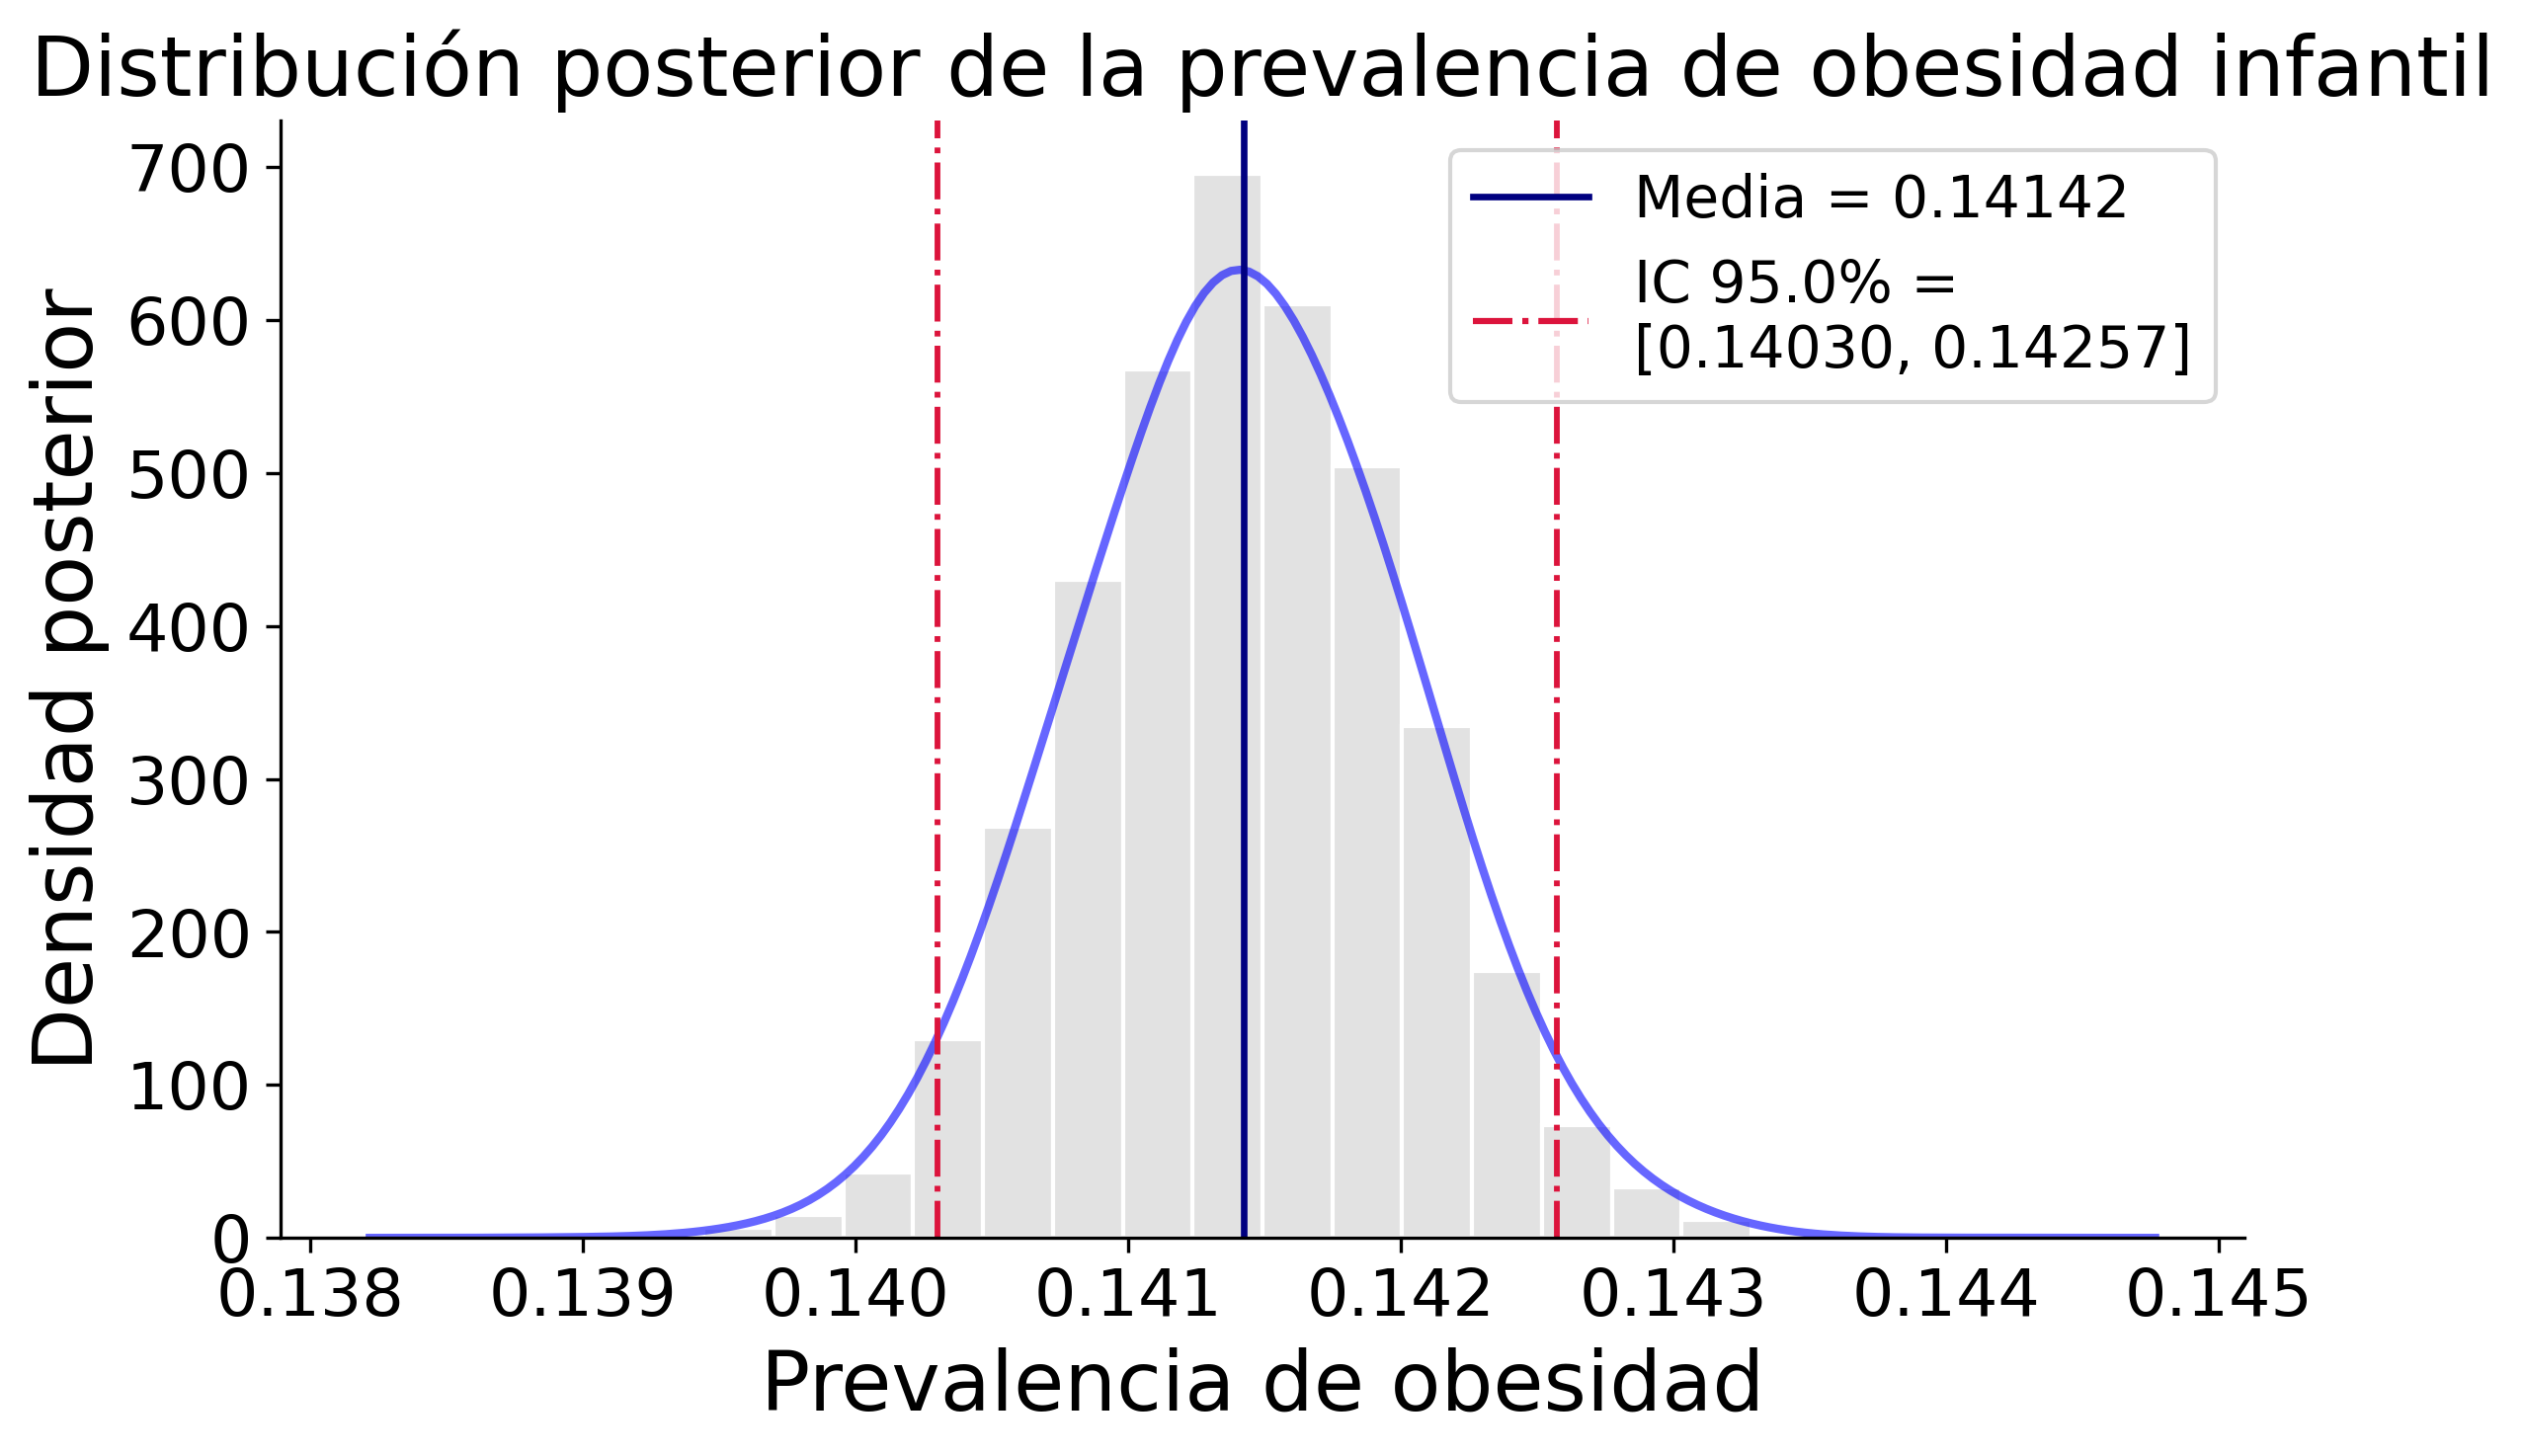
\includegraphics[width=0.7\linewidth]{../res/graficos/hist_post_obesidad} 

}

\caption{Distribución posterior de la prevalencia de obesidad infantil}\label{fig:fig-obesidad}
\end{figure}

Los histogramas permiten identificar distribuciones relativamente
simétricas para variables como años de escolaridad, hogares
monomarentales y ocupantes por hogar, mientras que otras como la
población urbana y la privación crítica presentan asimetrías y valores
extremos.

En cuanto a las asociaciones bivariadas, se observan patrones
relevantes:

\begin{itemize}
\item
  Existe una relación positiva entre la prevalencia de
  sobrepeso/obesidad y los años de escolaridad promedio (los distritos
  con mayor escolaridad tienden a reportar mayor prevalencia).
\item
  La relación con la tasa de desempleo es débil y ligeramente negativa,
  indicando que este factor no parece estar fuertemente vinculado con la
  prevalencia.
\item
  El porcentaje de población urbana muestra una asociación positiva con
  la prevalencia, aunque con dispersión considerable.
\end{itemize}

Finalmente, al comparar por provincia, la prevalencia combinada oscila
entre 30\% en Limón y 37\% en Heredia, siendo esta última la más alta.
Los boxplots confirman una mayor heterogeneidad en provincias como San
José y Alajuela, mientras que Cartago y Guanacaste presentan
distribuciones más concentradas.

\subsection{Fundamento Teórico}\label{fundamento-teuxf3rico}

\subsubsection{Hamiltonian Monte Carlo}\label{hamiltonian-monte-carlo}

Hamiltonian Monte Carlo (HMC) es un método de Monte Carlo por cadenas de
Markov que introduce variables auxiliares de momento para transformar el
muestreo de la distribución posterior \(p(\theta\mid y)\) en la
integración de un sistema hamiltoniano. Se define la energía potencial
\(U(\theta)=-\log p(\theta\mid y)\) y la energía cinética
\(K(r)=\tfrac12 r^\top M^{-1} r\) para un vector de momentos \(r\) y una
matriz de masa \(M\). La dinámica hamiltoniana preserva volumen y
energía, y se aproxima con el integrador leapfrog, que usa un tamaño de
paso \(\epsilon\) y un número de pasos \(L\) para proponer estados
\(\theta^*,r^*)\) alejados del estado actual, evitando la caminata
aleatoria. La propuesta se corrige con un paso de aceptación Metropolis
con probabilidad \(\min\{1,\exp[-\Delta H]\}\), donde \(\Delta H\) es el
cambio en la energía debido a la discretización. Esta construcción
aprovecha gradientes del log-posterior, permitiendo trayectorias largas
con baja autocorrelación y alto tamaño efectivo de muestra por
evaluación del gradiente. En la práctica, el rendimiento depende de
sintonizar \(\epsilon\), \(L\) y \(M\); tamaños de paso demasiado
grandes inducen divergencias, mientras que tamaños de paso muy pequeños
incrementan el costo computacional. La literatura recomienda adaptar
\(\epsilon\) hacia una tasa de aceptación objetivo y adaptar \(M\)
(diagonal o densa) para adecuar la escala y curvatura del posterior,
mejorando la estabilidad y la mezcla de la cadena
(\citeproc{ref-HoffmanGelman2014}{Hoffman \& Gelman, 2014}).

\subsubsection{NUTS}\label{nuts}

El No-U-Turn Sampler (NUTS) es una extensión adaptativa de HMC que
elimina la necesidad de fijar manualmente la longitud de trayectoria. En
lugar de elegir un \(L\) fijo, NUTS expande dinámicamente la trayectoria
(mediante un árbol binario) hasta detectar una no-u-turn: el punto en
que la dirección del movimiento comienza a invertirse y proseguir
añadiría recorrido redundante. Esta regla de detención garantiza
trayectorias lo suficientemente largas para explorar eficientemente la
masa de probabilidad, pero no tan largas como para desperdiciar cómputo,
reduciendo la autocorrelación sin requerir sintonía manual de \(L\)
(\citeproc{ref-HoffmanGelman2014}{Hoffman \& Gelman, 2014, p. 3},
p.~10). En paralelo, NUTS emplea dual averaging para adaptar el tamaño
de paso \(\epsilon\) hacia una tasa de aceptación objetivo (usualmente
entre 0.8 y 0.95), lo que disminuye la incidencia de divergencias en
posteriors con alta curvatura. En modelos con enlace logit y covariables
estandarizadas ---como el logit-binomial descrito--- los gradientes
están bien definidos y escalados, de modo que NUTS puede construir
trayectorias estables que recorren el posterior con bajo error de
integración y buena mezcla entre cadenas. La combinación de la expansión
sin u-turn y la adaptación de \(\epsilon\) produce un muestreo eficiente
y reproducible, con diagnósticos de convergencia favorables (\(\hat{R}\)
cercano a 1 y tamaños efectivos altos), en línea con las recomendaciones
metodológicas de Hoffman \& Gelman
(\citeproc{ref-HoffmanGelman2014}{2014}).

\subsubsection{Logit-binomial}\label{logit-binomial}

El modelo logit-binomial describe conteos de ``éxitos'' \(y_i\) sobre
exposiciones \(n_i\) mediante una verosimilitud binomial y un enlace
logit para la probabilidad \(p_i\): \[
y_i \sim \mathrm{Binomial}(n_i, p_i),\qquad
\mathrm{logit}(p_i)=\eta_i=\alpha + X_i^\top\beta.
\] La función logit es
\(\mathrm{logit}(p)=\log\!\big(\tfrac{p}{1-p}\big)\) y su inversa es \[
p_i=\frac{\exp(\eta_i)}{1+\exp(\eta_i)}.
\] Condicionalmente en \(p_i\), la media y varianza de \(y_i\) son \[
\mathbb E[y_i\mid p_i]=n_i p_i,\qquad \mathrm{Var}(y_i\mid p_i)=n_i p_i(1-p_i).
\]

El intercepto \(\alpha\) es el log-odds cuando \(X_i=0\). Si las
covariables están estandarizadas, \(X_i=0\) representa un ``individuo
medio'' y \(\mathrm{logit}^{-1}(\alpha)\) es su probabilidad base. Cada
\(\beta_k\) representa el cambio en log-odds por un incremento de una
unidad en la covariable \(k\); si \(X\) está estandarizada, esto
equivale a un cambio de 1 desviación estándar. En términos de odds
ratio, \[
\text{OR}_k=\exp(\beta_k),
\] de modo que un aumento de 1 DE en \(X_{ik}\) multiplica las odds por
\(\exp(\beta_k)\).

En la escala logit los parámetros son no acotados. Usar
\(\alpha,\beta_j\sim\mathcal N(0,5)\) coloca un 95 por ciento previo
aproximadamente en \([-9.8,9.8]\) para cada coeficiente, lo que en odds
ratio equivale a \([\exp(-9.8),\exp(9.8)]\), abarcando varios órdenes de
magnitud. Con \(X\) estandarizada, esto constituye una prior débil
porque apenas restringe la probabilidad base y los efectos covariables,
dejando que la verosimilitud determine la magnitud de \(p_i\) y de
\(\beta\). Sin estandarización, la misma \(\mathcal N(0,5)\) podría no
ser débil si las unidades de \(X\) fueran muy grandes.

A partir de muestras posteriores \(\{p_i^{(s)}\}\), las réplicas
predictivas se generan como
\(\tilde y_i^{(s)}\sim\mathrm{Binomial}(n_i,p_i^{(s)})\). Con ellas se
evalúan calibración y ajuste mediante coberturas de intervalos creíbles,
MAE o RMSE entre proporciones observadas \(y_i/n_i\) y estimadas
\(p_i\). La linealidad en la escala logit y la varianza binomial son
supuestos centrales; si hubiera sobre-dispersión sistemática no
explicada por \(X\), puede ampliarse el modelo con términos jerárquicos
o estructuras espaciales que introduzcan correlación y pooling parcial
entre unidades.

\subsection{Explicación del Modelo}\label{explicaciuxf3n-del-modelo}

El estudio emplea un modelo logit-binomial para estimar la prevalencia
\(p_i\) a partir de conteos \(y_i\) sobre exposiciones \(n_i\), con
\(\mathrm{logit}(p_i)=\alpha+X_i^{\top}\beta\) y covariables previamente
estandarizadas. Las priors \(\alpha,\beta_j\sim\mathcal N(0,5)\) se
especifican en la escala log-odds y, al ser muy dispersas, actúan como
priors débiles. Antes del ajuste bayesiano se implementó una
optimización del conjunto de covariables mediante una búsqueda
exhaustiva de subconjuntos en un modelo lineal clásico, seleccionando el
que minimiza el criterio de información de Akaike (AIC); este paso
reduce la dimensionalidad del diseño \(X_i\), evita modelos
innecesariamente complejos y concentra el modelo logit--binomial en
aquellas covariables con mayor respaldo empírico según el AIC. La
inferencia se realiza con No-U-Turn Sampler (NUTS), un algoritmo HMC que
adapta automáticamente el tamaño de paso y la longitud efectiva de la
trayectoria, expandiéndola hasta detectar una ``no-u-turn''; este
procedimiento mejora la exploración del posterior al reducir la
autocorrelación y evita fijar manualmente el número de pasos de
integración, de acuerdo a Hoffman \& Gelman
(\citeproc{ref-HoffmanGelman2014}{2014}). El resultado son muestras
posteriores mezcladas para \(p_i\) y para \((\alpha,\beta)\), a partir
de las cuales se obtienen medias e intervalos de credibilidad por
provincia y agregados ponderados por \(n_i\) para país.

\subsubsection{Significado de los
parámetros}\label{significado-de-los-paruxe1metros}

\(\alpha\): es el intercepto en escala logit. Como las covariables se
estandarizan, \(\alpha\) representa el log-odds de la condición cuando
todas las covariables estandarizadas valen \(0\), es decir, en un
``distrito promedio'' (cada covariable en su media original). En la
escala de probabilidad, la prevalencia basal asociada es \[
p_0 = \mathrm{logit}^{-1}(\alpha) = \frac{1}{1 + e^{-\alpha}}.
\]

\(\beta_k\): es el efecto de la covariable \(k\) sobre el logit de la
prevalencia. Como \(X_k\) está estandarizada, \(\beta_k\) mide el cambio
en el log-odds al aumentar la covariable \(k\) en \(+1\) desviación
estándar, manteniendo las demás covariables fijas. En términos de odds,
\(\exp(\beta_k)\) es el factor multiplicativo sobre las odds de la
condición cuando \(X_k\) aumenta en \(+1\) DE; por ejemplo,
\(\exp(\beta_k)=1.2\) implica un aumento del 20 \% en las odds.

\(p_i\): es la probabilidad (prevalencia) de la condición en la fila
\(i\), es decir, la probabilidad de que una persona del distrito \(i\)
presente la condición dado su vector de covariables. Es la cantidad
central del modelo: determina la distribución binomial
\(y_i\mid p_i\sim\mathrm{Binomial}(n_i,p_i)\) y a partir de sus muestras
posteriores se obtienen medias, intervalos de credibilidad e indicadores
agregados (por provincia o país).

\subsubsection{Supuestos y
consecuencias}\label{supuestos-y-consecuencias}

Binomialidad: \(y_i\mid p_i \sim \mathrm{Binomial}(n_i,p_i)\) con
\(\mathrm{Var}(y_i\mid p_i)=n_i p_i(1-p_i)\).\\
Linealidad en logit: la relación entre covariables y \(p_i\) es lineal
en la escala logit.\\
Priors débiles: \(\mathcal N(0,5)\) deja que los datos dominen, salvo en
celdas con poca exposición.

\subsubsection{Validación empírica
reportada}\label{validaciuxf3n-empuxedrica-reportada}

Convergencia: \(\hat{R}=1.00\) en obesidad y sobrepeso; tamaños
efectivos mínimos en núcleo/colas superiores a 4700, lo que sugiere
exploración homogénea del posterior.\\
Precisión predictiva: obesidad con \(\mathrm{MAE}=0.023\) y
\(\mathrm{RMSE}=0.032\); sobrepeso con \(\mathrm{MAE}=0.021\) y
\(\mathrm{RMSE}=0.030\). Diferencias promedio entre proporciones
observadas y estimadas en el rango 2--3 puntos porcentuales.\\
Cobertura (IC95 \%): 77.8 \% para obesidad y 89.1 \% para sobrepeso.
Indica buena reproducción de la variabilidad; ligera subcobertura en
obesidad (estimaciones algo más concentradas), calibración más cercana
al nominal en sobrepeso.

\subsubsection{Resumen ejecutivo}\label{resumen-ejecutivo}

Es un modelo logit--binomial bayesiano con priors débiles; la inferencia
usa NUTS (HMC) con adaptación automática para explorar eficientemente la
posterior. El script estandariza covariables, selecciona un subconjunto
mediante AIC, estima el modelo, resume \(p_i\) por fila y agrega
provincias/país ponderando por la exposición, además de graficar
distribuciones posteriores comparables entre provincias. El resultado es
un flujo reproducible para cuantificar prevalencias y su incertidumbre a
distintos niveles territoriales, con métricas de desempeño que respaldan
la calidad del ajuste. Como complemento a este informe, se desarrolló un
dashboard interactivo, el cual se ejecuta de manera local dentro del
entorno del proyecto de acuerdo a las instrucciones disponibles en el
README del \href{https://github.com/CA0307-II-2025/grupo-1}{repositorio}

\section{Resultados}\label{resultados}

\begin{figure}[H]

{\centering 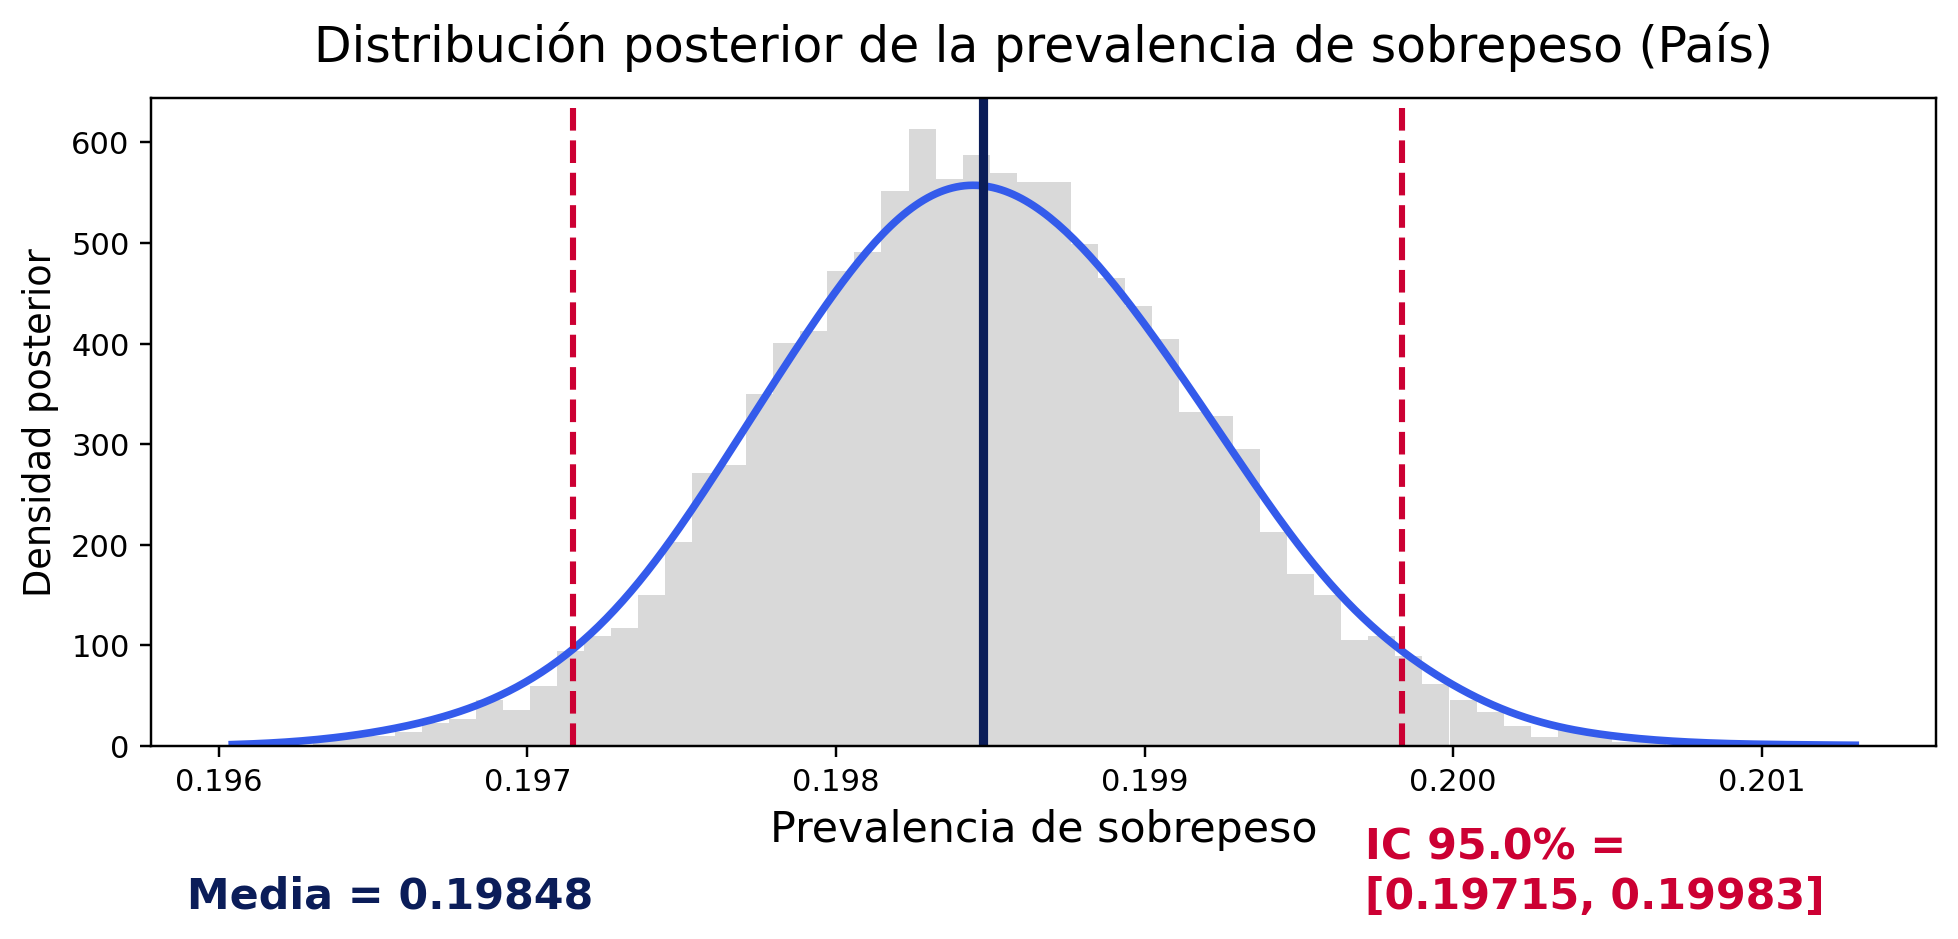
\includegraphics[width=0.7\linewidth]{../res/graficos/graficos_simulados_no_jer/sobrepeso/posterior_prevalencia_sobrepeso_pais} 

}

\caption{Distribución posterior de la prevalencia de sobrepeso infantil a nivel país}\label{fig:fig-mosaico_sobrepeso}
\end{figure}
\begin{figure}[H]

{\centering 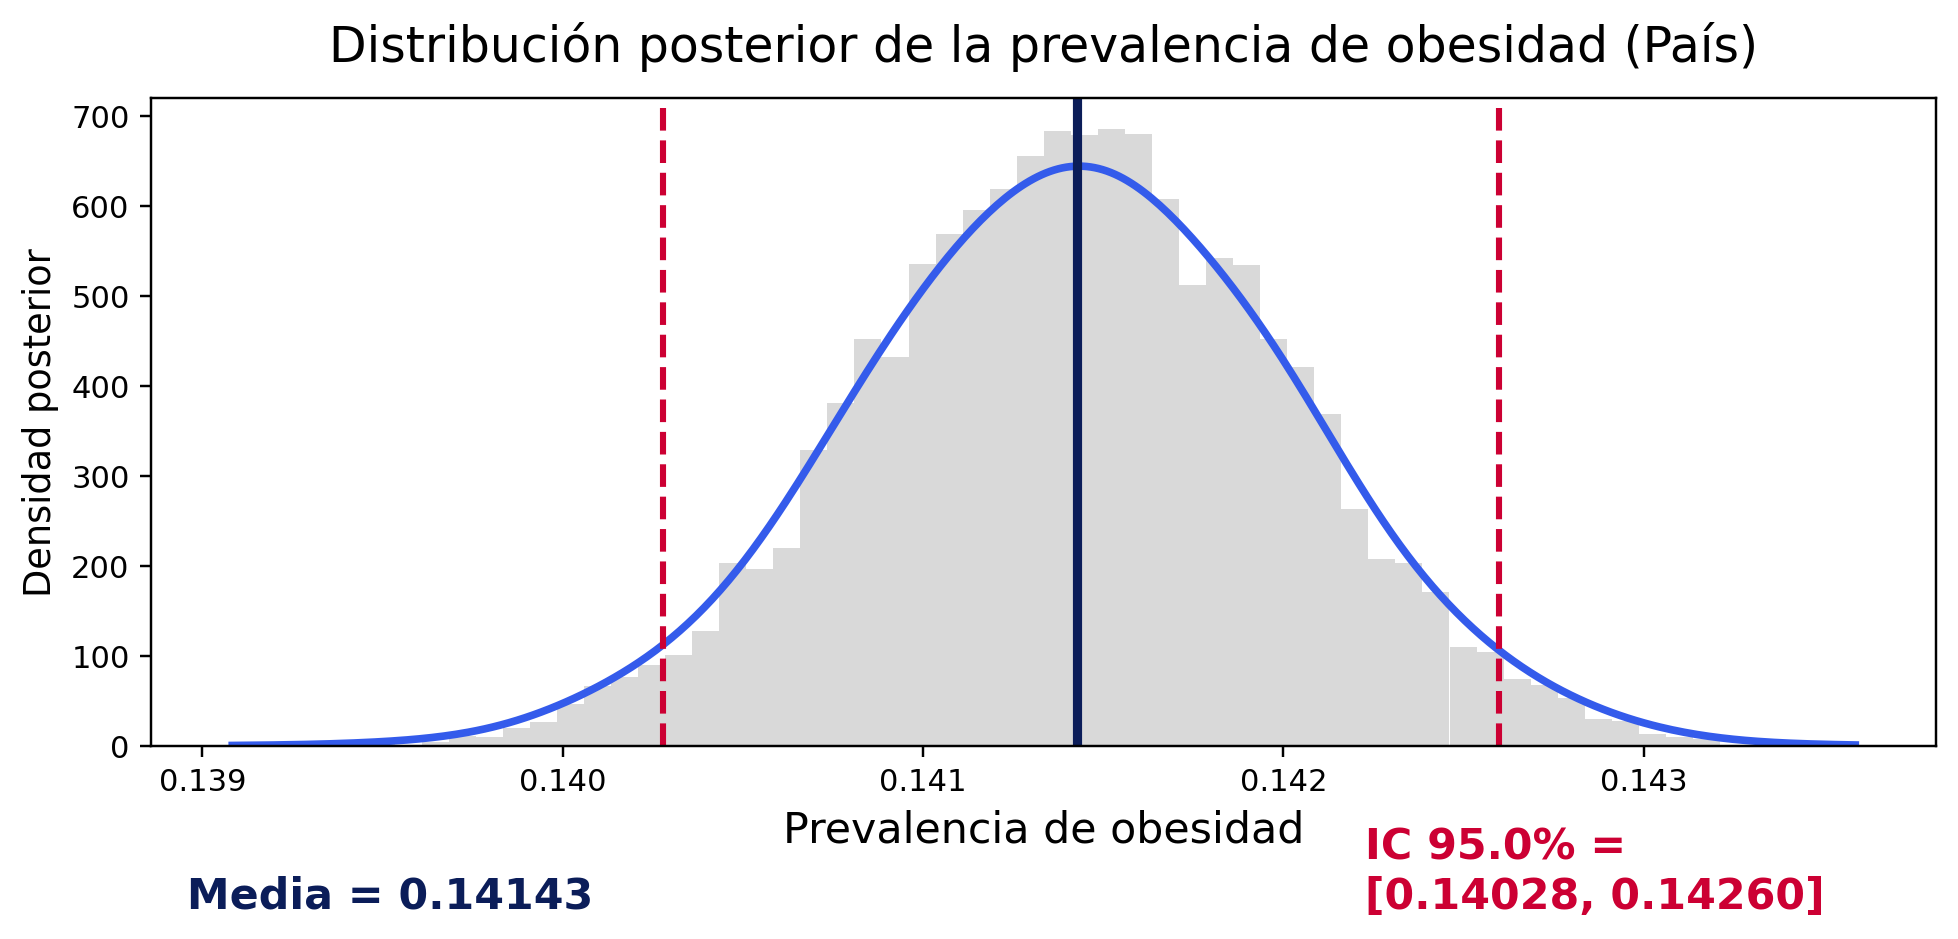
\includegraphics[width=0.7\linewidth]{../res/graficos/graficos_simulados_no_jer/obesidad/posterior_prevalencia_obesidad_pais} 

}

\caption{Distribución posterior de la prevalencia de obesidad infantil a nivel país}\label{fig:fig-mosaico_obesidad}
\end{figure}

\begin{longtable}[]{@{}
  >{\centering\arraybackslash}p{(\linewidth - 8\tabcolsep) * \real{0.1395}}
  >{\centering\arraybackslash}p{(\linewidth - 8\tabcolsep) * \real{0.1860}}
  >{\centering\arraybackslash}p{(\linewidth - 8\tabcolsep) * \real{0.2326}}
  >{\centering\arraybackslash}p{(\linewidth - 8\tabcolsep) * \real{0.1977}}
  >{\centering\arraybackslash}p{(\linewidth - 8\tabcolsep) * \real{0.2442}}@{}}
\caption{Resumen por provincia: obesidad y sobrepeso}\tabularnewline
\toprule\noalign{}
\begin{minipage}[b]{\linewidth}\centering
Grupo
\end{minipage} & \begin{minipage}[b]{\linewidth}\centering
Media\_Obesidad
\end{minipage} & \begin{minipage}[b]{\linewidth}\centering
Intervalo Obesidad
\end{minipage} & \begin{minipage}[b]{\linewidth}\centering
Media\_Sobrepeso
\end{minipage} & \begin{minipage}[b]{\linewidth}\centering
Intervalo Sobrepeso
\end{minipage} \\
\midrule\noalign{}
\endfirsthead
\toprule\noalign{}
\begin{minipage}[b]{\linewidth}\centering
Grupo
\end{minipage} & \begin{minipage}[b]{\linewidth}\centering
Media\_Obesidad
\end{minipage} & \begin{minipage}[b]{\linewidth}\centering
Intervalo Obesidad
\end{minipage} & \begin{minipage}[b]{\linewidth}\centering
Media\_Sobrepeso
\end{minipage} & \begin{minipage}[b]{\linewidth}\centering
Intervalo Sobrepeso
\end{minipage} \\
\midrule\noalign{}
\endhead
\bottomrule\noalign{}
\endlastfoot
Alajuela & 0.14096 & {[}0.13957, 0.14236{]} & 0.19873 & {[}0.19714,
0.20029{]} \\
Cartago & 0.14648 & {[}0.1451, 0.14789{]} & 0.20347 & {[}0.20194,
0.20497{]} \\
Guanacaste & 0.13749 & {[}0.13594, 0.13907{]} & 0.19000 & {[}0.18815,
0.19185{]} \\
Heredia & 0.14832 & {[}0.14671, 0.14995{]} & 0.20699 & {[}0.2053,
0.20869{]} \\
Limon & 0.12645 & {[}0.12465, 0.12827{]} & 0.18394 & {[}0.18187,
0.18604{]} \\
Puntarenas & 0.12810 & {[}0.12668, 0.12952{]} & 0.19135 & {[}0.18964,
0.19305{]} \\
San Jose & 0.14892 & {[}0.14753, 0.1503{]} & 0.20379 & {[}0.20218,
0.20535{]} \\
Pais & 0.14143 & {[}0.14025, 0.14258{]} & 0.19847 & {[}0.19708,
0.19978{]} \\
\end{longtable}

\begin{longtable}[]{@{}
  >{\centering\arraybackslash}p{(\linewidth - 8\tabcolsep) * \real{0.1685}}
  >{\centering\arraybackslash}p{(\linewidth - 8\tabcolsep) * \real{0.1798}}
  >{\centering\arraybackslash}p{(\linewidth - 8\tabcolsep) * \real{0.2247}}
  >{\centering\arraybackslash}p{(\linewidth - 8\tabcolsep) * \real{0.1910}}
  >{\centering\arraybackslash}p{(\linewidth - 8\tabcolsep) * \real{0.2360}}@{}}
\caption{Resumen por cantones más relevantes: obesidad y
sobrepeso}\tabularnewline
\toprule\noalign{}
\begin{minipage}[b]{\linewidth}\centering
Grupo
\end{minipage} & \begin{minipage}[b]{\linewidth}\centering
Media\_Obesidad
\end{minipage} & \begin{minipage}[b]{\linewidth}\centering
Intervalo Obesidad
\end{minipage} & \begin{minipage}[b]{\linewidth}\centering
Media\_Sobrepeso
\end{minipage} & \begin{minipage}[b]{\linewidth}\centering
Intervalo Sobrepeso
\end{minipage} \\
\midrule\noalign{}
\endfirsthead
\toprule\noalign{}
\begin{minipage}[b]{\linewidth}\centering
Grupo
\end{minipage} & \begin{minipage}[b]{\linewidth}\centering
Media\_Obesidad
\end{minipage} & \begin{minipage}[b]{\linewidth}\centering
Intervalo Obesidad
\end{minipage} & \begin{minipage}[b]{\linewidth}\centering
Media\_Sobrepeso
\end{minipage} & \begin{minipage}[b]{\linewidth}\centering
Intervalo Sobrepeso
\end{minipage} \\
\midrule\noalign{}
\endhead
\bottomrule\noalign{}
\endlastfoot
Talamanca & 0.10117 & {[}0.09779, 0.1046{]} & 0.17762 & {[}0.17413,
0.18114{]} \\
Buenos Aires & 0.11142 & {[}0.10907, 0.11383{]} & 0.18071 & {[}0.17787,
0.18356{]} \\
Los Chiles & 0.11245 & {[}0.11006, 0.1149{]} & 0.17539 & {[}0.17254,
0.17824{]} \\
La Cruz & 0.11639 & {[}0.11439, 0.11842{]} & 0.18108 & {[}0.17874,
0.18344{]} \\
Matina & 0.11767 & {[}0.11545, 0.11994{]} & 0.17928 & {[}0.17661,
0.1819{]} \\
Heredia & 0.15713 & {[}0.15495, 0.15935{]} & 0.21262 & {[}0.21051,
0.21465{]} \\
Santo Domingo & 0.15720 & {[}0.15501, 0.15938{]} & 0.21487 & {[}0.21239,
0.2173{]} \\
Moravia & 0.15842 & {[}0.15617, 0.16073{]} & 0.21311 & {[}0.21097,
0.2152{]} \\
Belen & 0.15857 & {[}0.15622, 0.16087{]} & 0.21879 & {[}0.21605,
0.22153{]} \\
Montes De Oca & 0.16897 & {[}0.16519, 0.17287{]} & 0.22065 & {[}0.2171,
0.22418{]} \\
\end{longtable}

Los resultados obtenidos a partir del modelo binomial con enlace logit y
muestreo NUTS evidencian un patrón claro en la distribución de la
prevalencia de obesidad y sobrepeso infantil en Costa Rica, tanto a
nivel nacional como provincial. En el plano nacional, la media posterior
estimada para obesidad fue de 0.14143, con un intervalo de credibilidad
del 95\% entre 0.14023 y 0.14254. En el caso del sobrepeso, la media
posterior fue de 0.19848, con un intervalo de credibilidad del 95\%
entre 0.19715 y 0.19983. Estos resultados, cuando se suman, permiten
inferir que aproximadamente un 34\% de la población infantil escolar del
país presenta exceso de peso, cifra que confirma la magnitud del
problema de salud pública y se encuentra alineada con las tendencias
observadas en contextos internacionales. La Organización Mundial de la
Salud World Health Organization (\citeproc{ref-WHO2025}{2025}) señala
que ``childhood obesity has become one of the most serious public health
challenges of the 21st century'', al estimar que más de 390 millones de
niños y adolescentes de entre 5 y 19 años en el mundo tienen sobrepeso u
obesidad. Esta cifra global se sitúa en torno al 20\% de esa población,
lo que significa que Costa Rica presenta una proporción ligeramente
superior al promedio global, aunque en consonancia con otros países de
ingreso medio y urbano consolidado.

El modelo, basado en inferencia bayesiana con el algoritmo No-U-Turn
Sampler (NUTS), generó distribuciones posteriores estables para cada
provincia. En el caso de la obesidad, los resultados revelan un
gradiente centro--periferia: San José, Heredia y Cartago muestran las
mayores prevalencias medias (0.14870, 0.14804 y 0.14584
respectivamente), mientras que Guanacaste, Puntarenas y Limón presentan
los valores más bajos (0.13516, 0.13037 y 0.12788). Este patrón se
repite para el sobrepeso, con Heredia, Cartago y San José nuevamente en
los primeros lugares (0.20765, 0.20648 y 0.20435 respectivamente) y
Guanacaste y Puntarenas en los últimos (0.19067 y 0.18830). A nivel
cantonal, se observa un contraste similar: cantones periféricos como
Talamanca (obesidad 0.10117; sobrepeso 0.17762), Buenos Aires, Los
Chiles, La Cruz y Matina se sitúan en la cola inferior de la
distribución, mientras que cantones del Gran Área Metropolitana como
Heredia (0.15713; 0.21262), Santo Domingo, Moravia, Belén y Montes De
Oca (0.16897; 0.22065) concentran las prevalencias medias más altas de
obesidad y sobrepeso.

\section{Conclusiones y
Recomendaciones}\label{conclusiones-y-recomendaciones}

Estos hallazgos coinciden con el análisis espacial bayesiano de Gómez et
al. (\citeproc{ref-Gomez2023}{2023}), quienes observaron que ``las
prevalencias más altas de sobrepeso y obesidad infantil se concentran en
el Valle Central, en distritos cabecera de provincia y en zonas
urbanizadas de mayor desarrollo económico''. La evidencia de
Hernández-Vásquez et al. (\citeproc{ref-Hernandez2016}{2016}) para Perú,
donde la obesidad infantil predomina en zonas urbanas y costeras frente
a regiones andinas y amazónicas, refuerza esta lectura regional: el
exceso de peso tiende a concentrarse en territorios de mayor desarrollo
económico y urbano. En el caso costarricense, este patrón se refleja
tanto a nivel provincial como cantonal, con valores medios de obesidad y
sobrepeso más altos en provincias centrales y cantones del Gran Área
Metropolitana, y niveles menores en provincias costeras y cantones
periféricos.

La consistencia de las distribuciones posteriores nacionales y
provinciales también se confirma al compararlas con las referencias
antropométricas nacionales de Núñez-Rivas et al.
(\citeproc{ref-Nunez2022}{2022}), quienes reportaron una prevalencia
combinada de sobrepeso y obesidad de 42.5\% en escolares costarricenses.
Aunque el presente modelo arroja una cifra ligeramente menor (≈34\%),
ello se puede deber a las diferencias en la definición de la muestra
(niños de 6--12 años del censo escolar) y por el uso de un enfoque
bayesiano ajustado a covariables sociodemográficas. En conjunto, los
resultados revelan una prevalencia combinada elevada y relativamente
homogénea entre provincias, lo que sugiere un fenómeno generalizado y
sostenido en el tiempo más que un problema focalizado en unos pocos
territorios.

A nivel global, los resultados nacionales se sitúan dentro del rango
descrito por la evidencia reciente. El Global Burden of Disease 2025
documenta que la prevalencia mundial de sobrepeso y obesidad infantil se
ha duplicado desde 1990 y proyecta que hacia 2050 alrededor del 15\% de
los niños de 5--14 años tendrán obesidad GBD 2025 Collaborators
(\citeproc{ref-GBD2025}{2025}). El World Obesity Atlas 2023 advierte que
la obesidad infantil podría duplicarse respecto a 2020 y acercarse a 400
millones de niños para 2035 World Obesity Federation
(\citeproc{ref-WorldObesity2023}{2023}), mientras que Zhang et al.
(\citeproc{ref-Zhang2024}{2024}) estiman que aproximadamente uno de cada
cinco niños y adolescentes a nivel mundial presenta exceso de peso. La
prevalencia nacional de obesidad infantil en Costa Rica (≈14\%) y de
sobrepeso (≈20\%) se alinea estrechamente con estas cifras y es
comparable a la reportada por el Centers for Disease Control and
Prevention (\citeproc{ref-CDC2022}{2022}) para Estados Unidos (19.7\% de
obesidad en la población de 2--19 años), lo que sitúa al país dentro del
grupo de naciones con un desafío sanitario de magnitud similar al de
países de alto ingreso.

Las interpretaciones institucionales ayudan a entender estos patrones.
La OMS subraya que ``the fundamental cause of obesity and overweight is
an energy imbalance between calories consumed and calories expended''
World Health Organization (\citeproc{ref-WHO2025}{2025}), mientras que
United Nations Children's Fund (\citeproc{ref-UNICEF2023}{2023})
describen un entorno global que combina alta disponibilidad de alimentos
ultraprocesados con una marcada disminución de la actividad física en la
niñez. Esta ``trampa'' alimentaria y de sedentarismo se refleja en la
distribución espacial observada: territorios más urbanizados muestran
mayores prevalencias, y el sobrepeso infantil tiende a evolucionar hacia
obesidad en la vida adulta, tal como advierte el Global Burden of
Disease 2025 cuando señala que ``overweight in childhood frequently
tracks into adult obesity, amplifying the long-term disease burden'' GBD
2025 Collaborators (\citeproc{ref-GBD2025}{2025}). En consecuencia, las
estimaciones provinciales sintetizan tanto el estado actual del exceso
de peso infantil en Costa Rica como el potencial acumulativo de riesgo
futuro en un entorno nacional que favorece dietas densas en energía y
menor actividad física.

Los resultadoss obtenidos confirman la existencia de una problemática
estructural de salud pública en plena expansión, con una prevalencia
combinada de sobrepeso y obesidad cercana al 34 \% y un patrón
geográfico que concentra los valores más altos en provincias y cantones
más urbanizados del Valle Central frente a las zonas costeras y
periféricas. La similitud de estas estimaciones con los hallazgos
internacionales y regionales muestra que el exceso de peso infantil
costarricense forma parte de un fenómeno global de gran escala y de
larga duración, en línea con las proyecciones de aumento sostenido de la
obesidad infantil documentadas por el Global Burden of Disease GBD 2025
Collaborators (\citeproc{ref-GBD2025}{2025}) y el World Obesity Atlas
World Obesity Federation (\citeproc{ref-WorldObesity2023}{2023}). De
esta manera, las estimaciones de este estudio proporcionan una base
empírica robusta para dimensionar la magnitud del problema en Costa Rica
y constituyen un punto de partida para el diseño de intervenciones
públicas y escolares basadas en evidencia, con especial énfasis en los
territorios urbanos de mayor riesgo.

Desde el punto de vista metodológico, los resultados presentan
consistencia y precisión aceptables en todos los niveles geográficos: el
uso de muestreo NUTS permitió explorar adecuadamente la distribución
posterior de los parámetros, reducir la autocorrelación entre cadenas y
alcanzar buena convergencia, lo que refuerza la confianza en los valores
reportados y en su comparabilidad futura. No obstante, y en línea con
las recomendaciones metodológicas de Gómez et al.
(\citeproc{ref-Gomez2023}{2023}), una agenda natural de trabajo es
extender el modelo hacia estructuras espaciales jerárquicas (por
ejemplo, especificaciones tipo BYM2) que capturen dependencia geográfica
residual y refinen las estimaciones en provincias y cantones con escasa
información, de modo que el sistema de vigilancia estadística del
sobrepeso y la obesidad infantil en Costa Rica pueda acompañar con mayor
precisión el diseño, la focalización y la evaluación de políticas
públicas.

\section{Referencias
Bibliográficas}\label{referencias-bibliogruxe1ficas}

\phantomsection\label{refs}
\begin{CSLReferences}{1}{0}
\bibitem[\citeproctext]{ref-CDC2022}
Centers for Disease Control and Prevention. (2022). \emph{Childhood
obesity facts}.

\bibitem[\citeproctext]{ref-Gamboa2021}
Gamboa-Gamboa, T., Fantin, R., Cordoba, J., Caravaca, I., \&
Gómez-Duarte, I. (2021). Relationship between childhood obesity and
socio-economic status among primary school children in costa rica.
\emph{Public Health Nutrition}, \emph{24}(12), 3825--3833.
\url{https://doi.org/10.1017/S1368980021002032}

\bibitem[\citeproctext]{ref-GBD2025}
GBD 2025 Collaborators. (2025). Global prevalence of child and
adolescent overweight and obesity, 1990--2021, with forecasts to 2050.
\emph{The Lancet}, \emph{405}(10345), 1--12.
\url{https://doi.org/10.1016/s0140-6736(25)00397-6}

\bibitem[\citeproctext]{ref-Gelfand2010Handbook}
Gelfand, A. E., Diggle, P. J., Guttorp, P., \& Fuentes, M. (Eds.).
(2010). \emph{Handbook of spatial statistics}. Chapman \& Hall/CRC.
\url{https://doi.org/10.1201/9781420072884}

\bibitem[\citeproctext]{ref-Gomez2023}
Gómez, M. J., Barboza, L. A., Vásquez, P., \& Moraga, P. (2023).
Bayesian spatial modeling of childhood overweight and obesity prevalence
in costa rica. \emph{BMC Public Health}, \emph{23}(1).
\url{https://doi.org/10.1186/s12889-023-15486-1}

\bibitem[\citeproctext]{ref-Hernandez2016}
Hernández-Vásquez, A., Bendezú-Quispe, G., Díaz-Seijas, D., Santero, M.,
Minckas, N., Azañedo, D., \& Antiporta, D. A. (2016). Análisis espacial
del sobrepeso y la obesidad infantil en el perú, 2014 {[}spatial
analysis of childhood obesity and overweight in peru, 2014{]}.
\emph{Revista Peruana de Medicina Experimental y Salud Pública},
\emph{33}(3), 489--497.
\url{https://doi.org/10.17843/rpmesp.2016.333.2298}

\bibitem[\citeproctext]{ref-HoffmanGelman2014}
Hoffman, M. D., \& Gelman, A. (2014). The no-u-turn sampler: Adaptively
setting path lengths in hamiltonian monte carlo. \emph{Journal of
Machine Learning Research}, \emph{15}, 1593--1623.
\url{https://www.jmlr.org/papers/v15/hoffman14a.html}

\bibitem[\citeproctext]{ref-Moraga2019Geospatial}
Moraga, P. (2019). \emph{Geospatial health data: Modeling and
visualization with r-INLA and shiny}. Chapman \& Hall/CRC.
\url{https://doi.org/10.1201/9780429341823}

\bibitem[\citeproctext]{ref-Moraga2020Sloth}
Moraga, P. (2020). Species distribution modeling using spatial point
processes: A case study of sloth occurrence in costa rica. \emph{The R
Journal}, \emph{12}(2), 293--310.
\url{https://doi.org/10.32614/RJ-2021-017}

\bibitem[\citeproctext]{ref-Moraga2023SpatialStats}
Moraga, P. (2023). \emph{Spatial statistics for data science: Theory and
practice with r}. Chapman \& Hall/CRC.
\url{https://doi.org/10.1201/9781032641522}

\bibitem[\citeproctext]{ref-Nunez2022}
Núñez-Rivas, H. P., Holst-Schumacher, I., Campos-Saborío, N., \&
López-López, E. (2022). Percentiles of body mass index and waist
circumference for costa rican children and adolescents. Percentiles de
índice de masa corporal y circunferencia de la cintura en niños y
adolescentes de costa rica. \emph{Nutrición Hospitalaria}, \emph{39}(6),
1228--1236. \url{https://doi.org/10.20960/nh.04130}

\bibitem[\citeproctext]{ref-UNICEF2023}
United Nations Children's Fund. (2023). \emph{Prevention of overweight
and obesity in children and adolescents: Programme guidance}.

\bibitem[\citeproctext]{ref-WHO2018}
World Health Organization. (2018). \emph{Taking action on childhood
obesity}.
\url{https://apps.who.int/iris/bitstream/handle/10665/274792/WHO-NMH-PND-ECHO-18.1-eng.pdf}.

\bibitem[\citeproctext]{ref-WHO2025}
World Health Organization. (2025). \emph{Obesity and overweight: Fact
sheet}.

\bibitem[\citeproctext]{ref-WorldObesity2023}
World Obesity Federation. (2023). \emph{World obesity atlas 2023}.

\bibitem[\citeproctext]{ref-Zhang2024}
Zhang, X., Wang, L., \& Liu, H. (2024). Global prevalence of overweight
and obesity in children and adolescents: A systematic review and
meta-analysis. \emph{JAMA Pediatrics}, \emph{178}(5), 1--12.
\url{https://doi.org/10.1001/jamapediatrics.2024.1576}

\end{CSLReferences}

\section{Anexos}\label{anexos}

\begin{longtable}[]{@{}
  >{\centering\arraybackslash}p{(\linewidth - 8\tabcolsep) * \real{0.2211}}
  >{\centering\arraybackslash}p{(\linewidth - 8\tabcolsep) * \real{0.1684}}
  >{\centering\arraybackslash}p{(\linewidth - 8\tabcolsep) * \real{0.2105}}
  >{\centering\arraybackslash}p{(\linewidth - 8\tabcolsep) * \real{0.1789}}
  >{\centering\arraybackslash}p{(\linewidth - 8\tabcolsep) * \real{0.2211}}@{}}
\caption{Resumen por cantones: obesidad y sobrepeso}\tabularnewline
\toprule\noalign{}
\begin{minipage}[b]{\linewidth}\centering
Grupo
\end{minipage} & \begin{minipage}[b]{\linewidth}\centering
Media\_Obesidad
\end{minipage} & \begin{minipage}[b]{\linewidth}\centering
Intervalo Obesidad
\end{minipage} & \begin{minipage}[b]{\linewidth}\centering
Media\_Sobrepeso
\end{minipage} & \begin{minipage}[b]{\linewidth}\centering
Intervalo Sobrepeso
\end{minipage} \\
\midrule\noalign{}
\endfirsthead
\toprule\noalign{}
\begin{minipage}[b]{\linewidth}\centering
Grupo
\end{minipage} & \begin{minipage}[b]{\linewidth}\centering
Media\_Obesidad
\end{minipage} & \begin{minipage}[b]{\linewidth}\centering
Intervalo Obesidad
\end{minipage} & \begin{minipage}[b]{\linewidth}\centering
Media\_Sobrepeso
\end{minipage} & \begin{minipage}[b]{\linewidth}\centering
Intervalo Sobrepeso
\end{minipage} \\
\midrule\noalign{}
\endhead
\bottomrule\noalign{}
\endlastfoot
Abangares & 0.14002 & {[}0.13746, 0.14272{]} & 0.18187 & {[}0.17856,
0.18532{]} \\
Acosta & 0.13513 & {[}0.13279, 0.13754{]} & 0.19586 & {[}0.19253,
0.19913{]} \\
Alajuela & 0.14993 & {[}0.14848, 0.15137{]} & 0.20433 & {[}0.20273,
0.20584{]} \\
Alajuelita & 0.13902 & {[}0.13771, 0.14035{]} & 0.19931 & {[}0.19699,
0.20164{]} \\
Alvarado & 0.13779 & {[}0.13467, 0.14101{]} & 0.20719 & {[}0.20421,
0.21019{]} \\
Aserri & 0.14252 & {[}0.1412, 0.14385{]} & 0.20003 & {[}0.19862,
0.20137{]} \\
Atenas & 0.14991 & {[}0.14764, 0.15214{]} & 0.20907 & {[}0.20645,
0.21173{]} \\
Bagaces & 0.13085 & {[}0.12948, 0.13223{]} & 0.18810 & {[}0.18635,
0.1898{]} \\
Barva & 0.15036 & {[}0.14798, 0.15273{]} & 0.21326 & {[}0.21083,
0.21567{]} \\
Belen & 0.15857 & {[}0.15622, 0.16087{]} & 0.21879 & {[}0.21605,
0.22153{]} \\
Buenos Aires & 0.11142 & {[}0.10907, 0.11383{]} & 0.18071 & {[}0.17787,
0.18356{]} \\
Carrillo & 0.13955 & {[}0.13694, 0.14225{]} & 0.18453 & {[}0.18168,
0.1875{]} \\
Cartago & 0.15106 & {[}0.14961, 0.15249{]} & 0.20672 & {[}0.20507,
0.20833{]} \\
Cañas & 0.13563 & {[}0.13421, 0.13701{]} & 0.19832 & {[}0.1964,
0.20027{]} \\
Corredores & 0.12164 & {[}0.11931, 0.124{]} & 0.19494 & {[}0.19229,
0.19757{]} \\
Coto Brus & 0.12038 & {[}0.11804, 0.12263{]} & 0.18857 & {[}0.18553,
0.19155{]} \\
Curridabat & 0.15153 & {[}0.14918, 0.15391{]} & 0.21138 & {[}0.20905,
0.21365{]} \\
Desamparados & 0.15327 & {[}0.15164, 0.15492{]} & 0.20427 & {[}0.20251,
0.20597{]} \\
Dota & 0.12525 & {[}0.12275, 0.12781{]} & 0.19638 & {[}0.19321,
0.19959{]} \\
El Guarco & 0.14634 & {[}0.14481, 0.14791{]} & 0.20285 & {[}0.20109,
0.20462{]} \\
Escazu & 0.15387 & {[}0.15175, 0.15606{]} & 0.21176 & {[}0.2095,
0.21395{]} \\
Esparza & 0.14310 & {[}0.14179, 0.14439{]} & 0.19959 & {[}0.19809,
0.20104{]} \\
Flores & 0.15471 & {[}0.15192, 0.15749{]} & 0.21564 & {[}0.21317,
0.21808{]} \\
Garabito & 0.13064 & {[}0.12908, 0.13216{]} & 0.19243 & {[}0.19046,
0.1944{]} \\
Goicoechea & 0.15535 & {[}0.15362, 0.1571{]} & 0.20649 & {[}0.20448,
0.20846{]} \\
Golfito & 0.12345 & {[}0.12161, 0.12535{]} & 0.18653 & {[}0.1844,
0.18862{]} \\
Grecia & 0.14654 & {[}0.14479, 0.14829{]} & 0.20229 & {[}0.20041,
0.20415{]} \\
Guacimo & 0.13137 & {[}0.12948, 0.13329{]} & 0.18534 & {[}0.18323,
0.18743{]} \\
Guatuso & 0.12292 & {[}0.12083, 0.12507{]} & 0.18721 & {[}0.18445,
0.19{]} \\
Heredia & 0.15713 & {[}0.15495, 0.15935{]} & 0.21262 & {[}0.21051,
0.21465{]} \\
Hojancha & 0.13769 & {[}0.1352, 0.14017{]} & 0.19812 & {[}0.19493,
0.20127{]} \\
Jimenez & 0.14469 & {[}0.14197, 0.14748{]} & 0.19989 & {[}0.19801,
0.20172{]} \\
La Cruz & 0.11639 & {[}0.11439, 0.11842{]} & 0.18108 & {[}0.17874,
0.18344{]} \\
La Union & 0.14868 & {[}0.14711, 0.15027{]} & 0.20540 & {[}0.20342,
0.20731{]} \\
Leon Cortes & 0.12654 & {[}0.12397, 0.12914{]} & 0.19546 & {[}0.19223,
0.1987{]} \\
Liberia & 0.13954 & {[}0.13694, 0.14214{]} & 0.19038 & {[}0.18791,
0.19287{]} \\
Limon & 0.12692 & {[}0.12409, 0.12975{]} & 0.18205 & {[}0.1794,
0.18472{]} \\
Los Chiles & 0.11245 & {[}0.11006, 0.1149{]} & 0.17539 & {[}0.17254,
0.17824{]} \\
Matina & 0.11767 & {[}0.11545, 0.11994{]} & 0.17928 & {[}0.17661,
0.1819{]} \\
Montes De Oca & 0.16897 & {[}0.16519, 0.17287{]} & 0.22065 & {[}0.2171,
0.22418{]} \\
Montes De Oro & 0.14516 & {[}0.1435, 0.14681{]} & 0.20547 & {[}0.20372,
0.20724{]} \\
Mora & 0.14789 & {[}0.14644, 0.14931{]} & 0.19757 & {[}0.19487,
0.20033{]} \\
Moravia & 0.15842 & {[}0.15617, 0.16073{]} & 0.21311 & {[}0.21097,
0.2152{]} \\
Nandayure & 0.14110 & {[}0.13788, 0.14447{]} & 0.18227 & {[}0.1784,
0.18627{]} \\
Naranjo & 0.14555 & {[}0.14357, 0.14757{]} & 0.20246 & {[}0.20057,
0.2043{]} \\
Nicoya & 0.13887 & {[}0.13707, 0.14067{]} & 0.19343 & {[}0.19117,
0.19568{]} \\
Oreamuno & 0.14284 & {[}0.14124, 0.14447{]} & 0.20584 & {[}0.20377,
0.20791{]} \\
Orotina & 0.13847 & {[}0.137, 0.13995{]} & 0.19699 & {[}0.19512,
0.19882{]} \\
Osa & 0.12323 & {[}0.12095, 0.12553{]} & 0.18917 & {[}0.18646,
0.19189{]} \\
Palmares & 0.15174 & {[}0.15002, 0.15343{]} & 0.20603 & {[}0.20435,
0.20768{]} \\
Paraiso & 0.14649 & {[}0.14454, 0.14847{]} & 0.19921 & {[}0.19774,
0.20062{]} \\
Parrita & 0.13311 & {[}0.13122, 0.13504{]} & 0.19314 & {[}0.19134,
0.19488{]} \\
Perez Zeledon & 0.13395 & {[}0.13273, 0.1352{]} & 0.19147 & {[}0.18984,
0.19306{]} \\
Poas & 0.14608 & {[}0.1443, 0.14789{]} & 0.19600 & {[}0.19415,
0.19785{]} \\
Pococi & 0.13402 & {[}0.13227, 0.13583{]} & 0.18629 & {[}0.18428,
0.18833{]} \\
Puntarenas & 0.13486 & {[}0.13359, 0.13611{]} & 0.19402 & {[}0.19245,
0.19557{]} \\
Puriscal & 0.14789 & {[}0.14581, 0.14995{]} & 0.19622 & {[}0.19269,
0.19985{]} \\
Quepos & 0.13772 & {[}0.13621, 0.13929{]} & 0.19031 & {[}0.18847,
0.19214{]} \\
San Carlos & 0.13096 & {[}0.12904, 0.13284{]} & 0.19314 & {[}0.19085,
0.19541{]} \\
San Isidro & 0.15440 & {[}0.15213, 0.15665{]} & 0.21693 & {[}0.21425,
0.2196{]} \\
San Jose & 0.15220 & {[}0.15028, 0.15419{]} & 0.20525 & {[}0.20291,
0.20758{]} \\
San Mateo & 0.13887 & {[}0.13659, 0.14112{]} & 0.19864 & {[}0.19569,
0.20157{]} \\
San Pablo & 0.15510 & {[}0.15212, 0.15811{]} & 0.21520 & {[}0.21286,
0.21749{]} \\
San Rafael & 0.15386 & {[}0.15188, 0.15581{]} & 0.20979 & {[}0.20769,
0.21185{]} \\
San Ramon & 0.14398 & {[}0.14259, 0.14536{]} & 0.19957 & {[}0.19764,
0.20147{]} \\
Santa Ana & 0.14753 & {[}0.14473, 0.15037{]} & 0.21331 & {[}0.21085,
0.21575{]} \\
Santa Barbara & 0.15008 & {[}0.14831, 0.15181{]} & 0.20963 & {[}0.20758,
0.21166{]} \\
Santa Cruz & 0.14334 & {[}0.14128, 0.1454{]} & 0.19022 & {[}0.18762,
0.1929{]} \\
Santo Domingo & 0.15720 & {[}0.15501, 0.15938{]} & 0.21487 & {[}0.21239,
0.2173{]} \\
Sarapiqui & 0.12051 & {[}0.11874, 0.12233{]} & 0.18089 & {[}0.17847,
0.18333{]} \\
Sarchi & 0.14647 & {[}0.14444, 0.14851{]} & 0.19619 & {[}0.19349,
0.19893{]} \\
Siquirres & 0.12822 & {[}0.12676, 0.12968{]} & 0.18880 & {[}0.18707,
0.19053{]} \\
Talamanca & 0.10117 & {[}0.09779, 0.1046{]} & 0.17762 & {[}0.17413,
0.18114{]} \\
Tarrazu & 0.13067 & {[}0.12911, 0.13226{]} & 0.19458 & {[}0.19276,
0.19642{]} \\
Tibas & 0.15626 & {[}0.15416, 0.15837{]} & 0.20752 & {[}0.20509,
0.20993{]} \\
Tilaran & 0.14055 & {[}0.1389, 0.14223{]} & 0.19843 & {[}0.19663,
0.20016{]} \\
Turrialba & 0.13858 & {[}0.13685, 0.14033{]} & 0.19674 & {[}0.19501,
0.19847{]} \\
Turrubares & 0.14667 & {[}0.1428, 0.1507{]} & 0.17948 & {[}0.1749,
0.18437{]} \\
Upala & 0.11776 & {[}0.11572, 0.11985{]} & 0.18586 & {[}0.18321,
0.1885{]} \\
Vazquez De Coronado & 0.15645 & {[}0.1547, 0.15819{]} & 0.21151 &
{[}0.20951, 0.21343{]} \\
Zarcero & 0.14198 & {[}0.13857, 0.1454{]} & 0.21224 & {[}0.20828,
0.21631{]} \\
Pais & 0.14143 & {[}0.14025, 0.14258{]} & 0.19847 & {[}0.19708,
0.19978{]} \\
\end{longtable}

\end{document}
